

\begin{figure}[H]
	\centering
	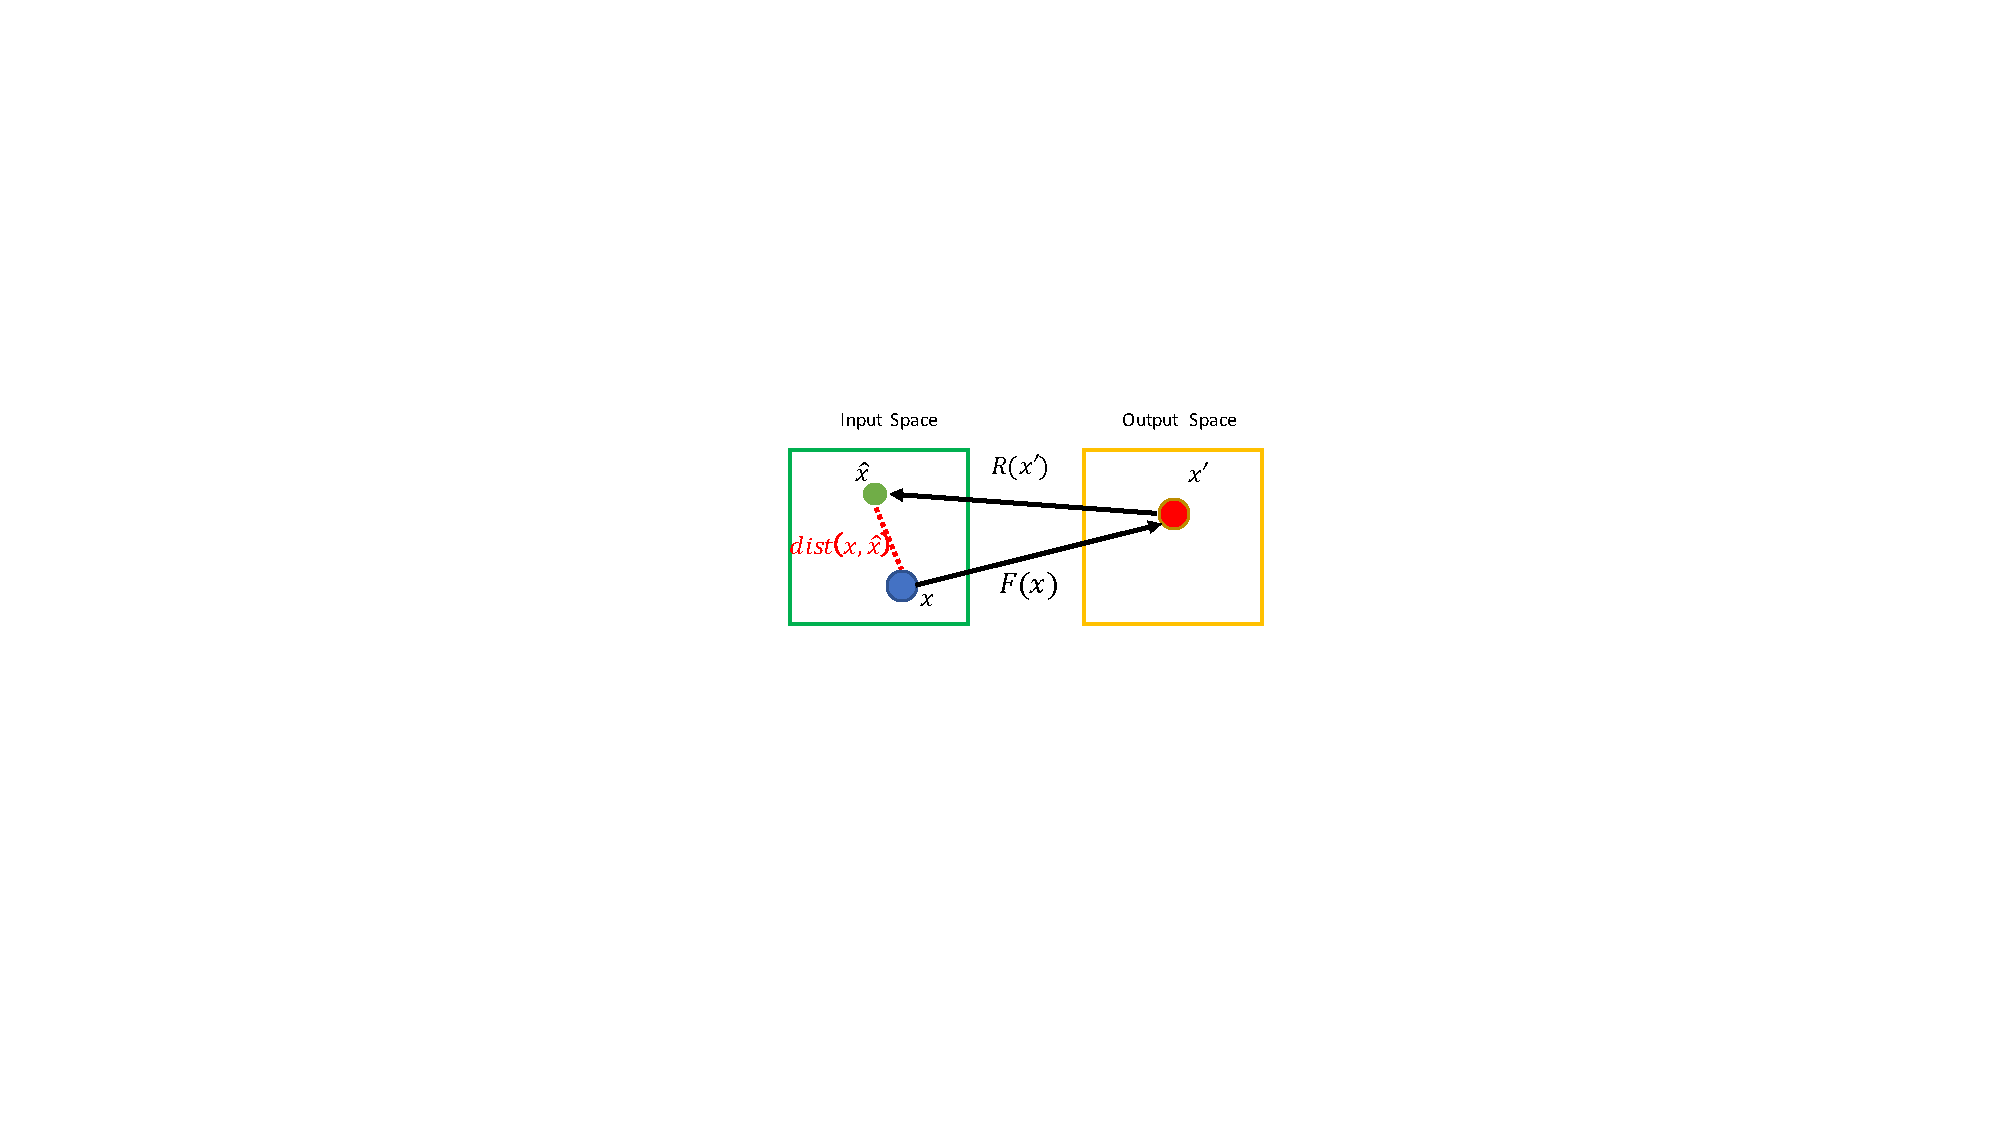
\includegraphics[width=0.4\textwidth]{\ChapterPathAutoGAN/figures/DR_P_CP}
	\caption{DR projection and reconstruction.} 
	\label{fig:DRP}
\end{figure} 

%\section{$\epsilon$-Dimension Reduction Privacy ($\epsilon$-DR Privacy)}
We introduce the Dimension Reduction Privacy (DR-Privacy), and define a formal definition of the $\epsilon$-DR Privacy to mathematically quantify/evaluate the mechanisms designed to preserve the DR-Privacy 
% the privacy that has been preserved
via dimension reduction. The DR-Privacy aims to achieve privacy-preserving via dimension reduction, which refers to transforming the data into a lower dimensional subspace, such that the private information is concealed while the underlying probabilistic characteristics are preserved, which can be utilized for machine learning purposes. To quantify the DR-Privacy and guide us to design such DR functions, we define $\epsilon$-DR Privacy as follows.


{\bf Definition 1}: ($\epsilon$-DR Privacy) A Dimension Reduction Function $F(\cdot)$ satisfies $\epsilon$-DR Privacy if for each i.i.d. $m$-dimension input sample $x$ drawn from the same distribution $D$, and for a certain distance measure $dist(\cdot)$, we have
\begin{equation}
\begin{split} \label{eq:modularity}
\mathbb{E}[dist(x, \hat{x})] \geq \epsilon
\end{split}
\end{equation}
where $\mathbb{E}[\cdot]$ is the expectation, $\epsilon \geq 0$, $x^{\prime}=F(x)$, $\hat{x}=R(x^{\prime})$, and $R(\cdot)$ is the Reconstruction Function.

For instance, as shown in Fig.~\ref{fig:DRP}, given original data $x$, our framework utilizes certain dimension reduction function $F(x)$ to transform the original data $x$ into the transformed data $x^{\prime}$. The adversaries aim to design a corresponding reconstruction function $R(x^{\prime})$ such that the reconstructed data $\hat{x}$ would be closed/similar to the original data $x$. DR-Privacy aims to design/develop such dimension reduction functions, that the distance between the original data and its reconstructed data would be large enough to protect the privacy of the data owner.

